\bookchapter{第四十九章：搭建開發環境——Android Studio 與第一個專案}

\chapterintro{工欲善其事，必先利其器。這一章咱們把“廚房”搭好：裝好 Android Studio、跑通模擬器、建立人生第一個安卓專案，再把工程結構拆開看個明白。裝好環境之後，你會第一次看到自己寫的程式碼變成一個能點的按鈕——這個瞬間，很多人會記一輩子。}

\booksection{一、安裝 Android Studio}

Android Studio 是谷歌官方的整合開發環境（IDE），免費，功能全家桶：寫程式碼、看介面預覽、除錯、打包全在裡面。安裝四步：

\begin{enumerate}
  \item 開啟官網 developer.android.com/studio，下載最新穩定版（2026 年 8 月是 Narwhal 之後的版本，Windows/Mac/Linux 都有）；
  \item 執行安裝包，一路"下一步"——安裝嚮導會自動帶上 Android SDK 和模擬器元件；
  \item 首次啟動時按提示下載 SDK 元件（預設勾選就好，可能需要幾分鐘和幾個 GB 的空間）；
  \item 完成後你會看到歡迎頁——恭喜，"廚房"搭好了。
\end{enumerate}

\begin{tcbwarn}{注意：硬體要求心裡有數}
Android Studio 是個“吃記憶體”的傢伙：建議 16GB 記憶體起步（8GB 也能跑，但模擬器一開會比較卡）、磁碟預留 20GB 以上、CPU 支援虛擬化（BIOS 裡開啟 VT-x/AMD-V）。如果電腦確實老舊，可以用“真機除錯”代替模擬器（本章第四節會講），體驗反而更流暢。

\end{tcbwarn}

\booksection{二、建立你的第一個專案}

在歡迎頁點 New Project，選 Empty Activity 模板（最乾淨的新手模板），然後填三樣東西：

\begin{center}
\begin{tabularx}{\linewidth}{|X|X|X|}
\hline
\textbf{配置項} & \textbf{填什麼} & \textbf{說明} \tabularnewline
\hline
Name & My First App & 應用程式名稱字，顯示在手機桌面上 \tabularnewline
Package name & com.example.myfirstapp & 全球唯一標識，習慣是"域名反寫"，先按預設 \tabularnewline
Minimum SDK & API 26（Android 8.0） & 最低支援版本，覆蓋 95\%+ 裝置 \tabularnewline
\hline
\end{tabularx}
\end{center}

\begin{center}\small\color{gray}建立專案要填的三件事\end{center}

點 Finish 後，Android Studio 會用 Gradle 自動下載依賴、構建專案（第一次要等幾分鐘，之後每次會快很多）。構建完成後，你就有了一個能跑的 App——雖然它還只會顯示一行“Hello Android!”。

\begin{tcbinfo}{小貼士：包名的門道}
包名（package name）就像 App 的“身份證號”，全球不能重複，上架後就不能改了。個人練習用 com.example.xxx 就行；正式產品要換成你自己的域名反寫（比如 com.你的名字.應用程式名稱）。別用 com.example 上架——商店會拒收。

\end{tcbinfo}

\booksection{三、跑起來：模擬器與真機}

程式碼寫好了，得找個“手機”來跑。你有兩個選擇：

\booksubsection{模擬器（Emulator）}

模擬器是在電腦裡虛擬出一臺安卓手機。在 Android Studio 裡開啟 Device Manager Create Device，挑一臺裝置（推薦 Pixel 系列） 選一個系統映象（帶 Google APIs 的） 下載 啟動。然後點工具欄的綠色三角 Run，幾秒鐘後，“手機”螢幕上就會出現你的 App。

\booksubsection{真機除錯（更推薦）}

真機永遠是最真實的測試環境——滑動手感、真網路、真感測器，模擬器都比不了。安卓真機除錯很簡單：

\begin{enumerate}
  \item 手機上開啟 [設定] [關於手機]，連點"版本號" 7 次，開啟"開發者選項"；
  \item 在 [開發者選項] 裡開啟 USB 除錯；
  \item 用資料線連電腦，手機跳出視窗選"允許 USB 除錯"；
  \item 回到 Android Studio，工具欄的裝置下拉選單裡就會出現你的手機，點 Run。
\end{enumerate}

\textbf{避坑提醒：USB 除錯別常開}\par

USB 除錯相當於給電腦開了“後門”。在公共場合充電、連線不信任的電腦時，務必關閉 USB 除錯，防止別人透過它讀取你的資料。平時開發用完就關，養成習慣。

\booksection{四、工程結構拆解：每個檔案是幹嘛的}

第一次開啟專案，左側的檔案樹可能讓你頭暈。別慌，日常開發你 90\% 的時間只跟下面這幾個打交道：

\begin{center}
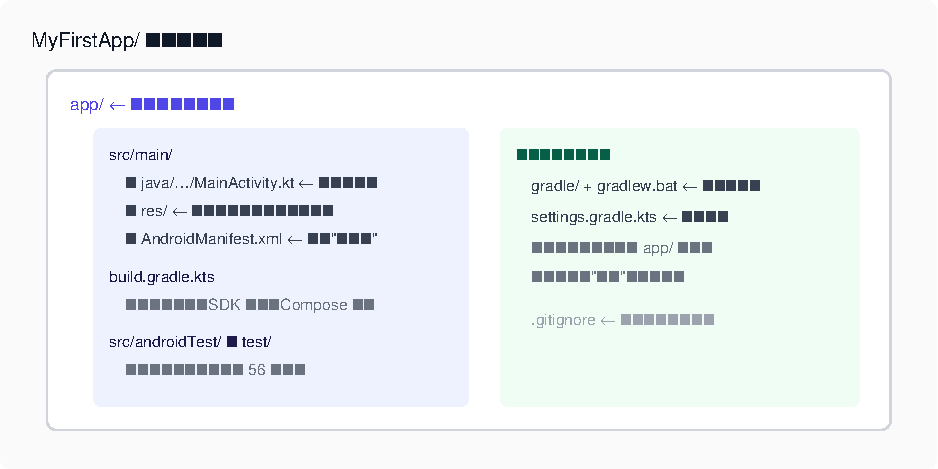
\includegraphics[width=0.92\linewidth]{figures/fig-di-si-shi-jiu-zhang-1}
\\[2pt]\small 圖 2：新手必懂的工程結構（口訣：只碰 app/ 目錄）
\end{center}

\begin{itemize}
  \item MainActivity.kt：App 的"大門"。使用者點開圖示，第一個被喚醒的就是它。現在的模板裡它負責顯示"Hello Android!"。
  \item AndroidManifest.xml：App 的"戶口本"——宣告這個 App 叫什麼、圖示是哪個、有哪些頁面、要用哪些權限（相機、定位等）。
  \item res/ 目錄：資源倉庫，存圖片、圖示、字串、顏色。把文字放資原始檔而不是寫死在程式碼裡，是安卓開發的好習慣（換語言、換主題都方便）。
  \item build.gradle.kts：構建配方——宣告最低支援版本、依賴哪些庫（比如 Compose）。
\end{itemize}

\booksection{五、小試牛刀：把“Hello”換成你的名字}

開啟 MainActivity.kt，你會看到 Compose 模板生成的程式碼。找到 Text(“Hello Android!”) 這一行，把引號裡的字換成你的名字，比如 Text(“你好，張三！這是我的第一個App”)，然後按 Ctrl+R（Mac 是 Cmd+R）重新執行。幾秒後，模擬器上就顯示了你的名字。

\begin{lstlisting}[language=Kotlin]
setContent {
    MyFirstAppTheme {
        Surface(modifier = Modifier.fillMaxSize()) {
            // v 把這裡改成你自己的文字
            Text("你好，張三！這是我的第一個App")
        }
    }
}
\end{lstlisting}

恭喜，你已經完成了一次完整的“改程式碼 編譯 安裝 執行”迴圈。這個迴圈，就是未來每一天的開發日常。趁熱打鐵，試著再改點別的：把字號調大、換個顏色——下一章我們就會學到這些“魔法”是怎麼來的。

\booksection{六、常見報錯急救：新手前兩週的“急診室”}

環境搭建和首次構建階段，你會大機率遇到下面三種報錯。別慌，都有解藥：

\begin{center}
\begin{tabularx}{\linewidth}{|X|X|X|}
\hline
\textbf{報錯現象} & \textbf{常見原因} & \textbf{解藥} \tabularnewline
\hline
Gradle sync failed / 依賴下載慢 & 網路訪問倉庫不暢 & 給 Gradle 配置國內映象倉庫（阿里雲/騰訊雲 maven 映象），網上搜"gradle 國內映象"照著改 \tabularnewline
SDK 元件缺失 & 安裝時跳過了 SDK 下載 & Settings SDK Manager 補裝缺失的平臺與工具 \tabularnewline
模擬器啟動失敗 / 黑屏 & 虛擬化未開啟、映象損壞 & BIOS 開 VT-x/AMD-V；刪掉模擬器重建；或直接用真機除錯 \tabularnewline
\hline
\end{tabularx}
\end{center}

\begin{center}\small\color{gray}新手環境報錯急救表\end{center}

\begin{tcbinfo}{小貼士：搜報錯的方法論}
報錯資訊第一行是最有價值的——把它原樣複製進搜尋引擎，加“android studio”關鍵字。別搜“我裝不上環境怎麼辦”這種籠統問題，搜“Gradle sync failed: Could not resolve com.android.tools.build”這種具體錯誤。精確的問題，才有精確的答案。

\end{tcbinfo}

\begin{tcbpractice}{來動手：完成你的"開發儀式感"清單}
(1) 裝好 Android Studio 並跑通模擬器；(2) 用真機跑一次自己的 App 並截圖留念；(3) 把 Hello 文字改成你的名字；(4) 把專案壓縮存個檔。做完這四步，你就可以在朋友圈宣佈：我也是安卓開發者了（截圖為證）。

\end{tcbpractice}

\begin{tcbsummary}{本章小結}
\begin{itemize}
  \item Android Studio = 官方免費 IDE；建議 16GB 記憶體 + 20GB 磁碟 + 開虛擬化
  \item 新增專案三要素：名字、包名（全球唯一，com.example 別上架）、最低 SDK（API 26 起）
  \item 兩種執行方式：模擬器（電腦裡虛擬手機）與真機（開 USB 除錯，用完記得關）
  \item 工程口訣：只碰 app/ 目錄——MainActivity.kt 是大門，Manifest 是戶口本，res/ 是資源倉庫
  \item 開發日常 = 改程式碼 Run 看效果，迴圈往復
\end{itemize}

\end{tcbsummary}
